%%%%%%%%%%%%%%%%%%%%%%%%%%%%%%%%%%%%%%%%%
% Professional Mathematical Presentation Template
% 
% This template uses the beamer class with the Madrid theme
% and a custom color scheme for a clean, professional look
% that works well with mathematical content.
%%%%%%%%%%%%%%%%%%%%%%%%%%%%%%%%%%%%%%%%%

\documentclass[aspectratio=169]{beamer} % 16:9 aspect ratio (modern)

% Theme settings
\usetheme{Madrid}
\usecolortheme{default}


\definecolor{primcolor}{RGB}{25,50,100} % Dark blue
\setbeamercolor{structure}{fg=primcolor}
\setbeamercolor{frametitle}{bg=primcolor!15, fg=primcolor}
\setbeamercolor{title}{fg=white} % White title text for contrast
\setbeamercolor{subtitle}{fg=white} % White subtitle text
\setbeamercolor{author}{fg=primcolor} % White author text
\setbeamercolor{date}{fg=primcolor} % White date text
\setbeamercolor{institute}{fg=primcolor} % White institute text

% Font settings
\usefonttheme{professionalfonts}
\usefonttheme{serif}

% Package imports
\usepackage{amsmath, amsfonts, amssymb, amsthm} % Math packages
\usepackage{mathtools} % Enhanced math tools
\usepackage{bm} % Bold math symbols
\usepackage{graphicx} % For images
\usepackage{booktabs} % Professional tables
\usepackage{tikz} % For diagrams
\usetikzlibrary{arrows, positioning, matrix, decorations.pathreplacing}

% Use beamer's theorem styles
\setbeamertemplate{theorem}[ams style]
\setbeamertemplate{theorems}[numbered]


% Remove navigation symbols
\setbeamertemplate{navigation symbols}{}

% Custom footer
\setbeamertemplate{footline}{
  \leavevmode%
  \hbox{%
  \begin{beamercolorbox}[wd=.333333\paperwidth,ht=2.25ex,dp=1ex,center]{author in head/foot}%
    \usebeamerfont{author in head/foot}\insertshortauthor
  \end{beamercolorbox}%
  \begin{beamercolorbox}[wd=.333333\paperwidth,ht=2.25ex,dp=1ex,center]{title in head/foot}%
    \usebeamerfont{title in head/foot}\insertshorttitle
  \end{beamercolorbox}%
  \begin{beamercolorbox}[wd=.333333\paperwidth,ht=2.25ex,dp=1ex,right]{date in head/foot}%
    \usebeamerfont{date in head/foot}\insertshortdate{}\hspace*{2em}
    \insertframenumber{} / \inserttotalframenumber\hspace*{2ex} 
  \end{beamercolorbox}}%
  \vskip0pt%
}

% Title information
\title[DP2]{Dynamic Programming}
\subtitle{Thomas J. Sargent and John Stachurski}
\author[Longye]{Longye Tian \\ \texttt{longye.tian@anu.edu.au}}
\institute[ANU]{Australian National University\\ School of Economics}
\date{March 7th, 2025}
\DeclareFontFamily{U}{mathx}{\hyphenchar\font45}
\DeclareFontShape{U}{mathx}{m}{n}{
      <5> <6> <7> <8> <9> <10>
      <10.95> <12> <14.4> <17.28> <20.74> <24.88>
      mathx10
      }{}
\DeclareSymbolFont{mathx}{U}{mathx}{m}{n}
\DeclareMathSymbol{\bigtimes}{1}{mathx}{"91}

\begin{document}

% Title frame
\begin{frame}
  \titlepage
\end{frame}

% Outline frame
\begin{frame}{Outline}
  \tableofcontents
\end{frame}
\section{3.1.1.1. Order Isomorphisms}
\begin{frame}{Order Isomorphism}
    
\end{frame}
\begin{frame}{Order Isomorphism}
\begin{definition}
    A surjective map $F$ from poset $(V,\precsim)$ to poset $(\hat V, \le)$ is called an 
    \begin{itemize}
        \item \textbf{Order isomorphism} if $v\precsim w\iff Fv\le Fw$
        \item \textbf{Order anti-isomorphism} if $v\precsim w \iff Fw\le Fv$
    \end{itemize}
\end{definition}
\textbf{Comment}: $F$ under this definition is bijective.
\end{frame}

\begin{frame}{Exercise 3.1.1.}
Given $h\in\mathbb{R}^X$, let $Fh = \exp(\theta h)$. Show that $F$ is an order isomorphism from $\mathbb{R}^X$ to $(0,\infty)^X$ whenever $\theta >0$.
\begin{proof}
    Fix $\theta>0$. We know that $\exp(\theta x)$ is a bijective function. 
    Let $h_1,h_2\in \mathbb{R}^X$ such that $h_1\le h_2$. This implies
    $$
    \theta h_1\le \theta h_2
    $$
    As $\exp(\cdot)$ is order preserving, hence, we have
    $$
    Fh_1  = \exp(\theta h_1) \le \exp(\theta h_2) = Fh_2
    $$
    Let $k_1, k_2\in (0,\infty)^X$, $k_1\le k_2$ by surjectivity, we have 
    $$
    k_1 = F(q_1) = \exp(\theta q_1), k_2 = F(q_2) = \exp(\theta q_2), q_1,q_2\in \mathbb{R}^X
    $$
\end{proof}
\end{frame}

\begin{frame}{Exercise 3.1.1. Continue}
\begin{proof}
    We have 
    $$
    q_1 = \frac{\ln k_1}{\theta}\le \frac{\ln k_2}{\theta} = q_2
    $$
    as $\ln$ is order preserving.
    Therefore, by definition, $F$ is an order isomorphism from $\mathbb{R}^X$ to $(0,\infty)^X$
\end{proof}    
\end{frame}

\begin{frame}{Exercise 3.1.2.}
Let $V= M^X$ and $\hat V = \hat M^X$, $M,\hat M\subset \mathbb{R}$. Let $\varphi$ be a map from $M$ onto $\hat M$ and let $Fv = \varphi\circ v$. Prove if $\varphi$ is an order isomorphism from $M$ to $\hat M$, then $F$ is an order isomorphism from $V$ to $\hat V$.
\begin{proof}
    $\varphi$ is order isomorphism then $\varphi$ is bijective, order preserving with order preserving inverse.
    Hence apply this $\dim X$ times, we get $F$ is bijective,  order preserving with order preserving inverse.
\end{proof}
    
\end{frame}

\begin{frame}{Exercise 3.1.3}
Let $V,\hat V$ be posets. Show that every order isomorphism $F$ is a bijection. Show that every order anti-isomorphism is also a bijection.
\begin{proof}
    Let $v_1,v_2\in \hat V$ such that $v_1 = v_2$. By surjectivity, we have
    $$
    v_1 = F(w_1), \quad v_2=F(w_2),\quad w_1,w_2\in V
    $$
    Hence, we have
    $$
    F(w_1)\le F(w_2) \implies w_1\precsim w_2
    $$
    $$
    F(w_2) \le F(w_1)\implies w_2\precsim w_1
    $$
    Hence,$w_1 = w_2$. This proves that $F$ is injective. 
\end{proof}
    
\end{frame}

\begin{frame}{Exercise 3.1.4.}
Let $F$ be a bijection from $(V,\precsim)$ to $(\hat V, \le)$. Show that
\begin{enumerate}
    \item $F$ is an order isomorphism if and only if $F$ and $F^{-1}$ are order preserving
    \item $F$ is an order anti-isomorphism if and only if $F$ and $F^{-1}$ are order reversing.
\end{enumerate}
\begin{proof}
    Skip
\end{proof}
\end{frame}

\begin{frame}{Lemma 3.1.1.}
Let $F$ be an order isomorphism from $(V,\precsim)$ to $(\hat V, \le)$. If the supremum of $\{v_\alpha\}_{\alpha\in \Lambda}\subset V$ exists in $V$, then
$$
\bigvee_{\alpha} Fv_\alpha \text{ exists in $\hat V$ and $\bigvee_\alpha Fv_\alpha = F\bigvee_\alpha v_\alpha$}
$$
\begin{proof}
    Let $v:= \bigvee_\alpha v_\alpha \in V$. Let $\hat w$ be any upper bound of $\{Fv_\alpha\}$, i.e., $Fv_\alpha \le \hat w$ for all $\alpha \in\Lambda$. By surjectivity, we let $\hat w = F(w)$, and by order isomorphism, we have
    $$
    v_\alpha \precsim w \quad \text{for all $\alpha\in\Lambda$}
    $$
    Hence, $w$ is an upper bound of $\{v_\alpha\}$, this implies $v\precsim w$. Hence, 
    $$
    F(v) \le F(w) =\hat w
    $$
    This implies $F(v)= F\bigvee_\alpha v_\alpha$ is the least upper bound of $\{Fv_\alpha\}$. 
\end{proof}
\end{frame}

\begin{frame}{Exercise 3.1.6}
Let $V,\hat V$ be posets and let $(v_n)$ be a sequence in $V$. And let $F$ be a map from $V$ to $\hat V$. Prove the following
\begin{enumerate}
    \item If $F$ is an order isomorphism, then $v_n\uparrow v$ if and only if $Fv_n \uparrow Fv$ in $\hat V$
    \item If $F$ is an order anti-isomorphism, then $v_n\uparrow v$ if and only if $Fv_n\downarrow Fv$ in $\hat V$.
\end{enumerate}
\begin{proof}
    $v_n\uparrow v\implies v_1\le v_2\le \cdots\le v$ and $v= \bigvee_n v_n$.\\
    Hence, by order isomorphism, we have
    $$
    Fv_1\le Fv_2\le \cdots \le Fv
    $$
    and $Fv = \bigvee_n Fv_n$
    Moreover, $F$ is order isomorphism implies $F^{-1}$ is order isomorphism. Hence, the other direction follows. 
\end{proof}
\end{frame}

\begin{frame}{Exercise 3.1.7}
Prove 
\begin{itemize}
    \item If $V,\hat V$ are order isomorphic, then $V$ is totally ordered if and only if $\hat V$ is totally ordered
    \item $F$ is an order anti-isomorphism from $V$ to $\hat V$ if and only if $F$ is an order isomorphism from $V$ to its dual $\hat V^\partial$
\end{itemize}
\begin{proof}
Skip.
\end{proof}
\end{frame}

\section{3.1.1.2 Conjugate Dynamics}
\begin{frame}{Conjugate Dynamics}
\begin{itemize}
    \item We start with the definition of conjugacy between dynamical systems ($(V, T_\sigma)$ is a dynamical system with state space $V$ and evolution $T_\sigma$).
    \item  Then, we go to the most basic structure, $V$ as a poset, and upgrade conjugacy to order conjugacy. 
    \item  This prepares for the later upgrade from dynamical system to ADP
\end{itemize}
\end{frame}
\begin{frame}{Definitions}
\begin{definition}
    We call a \textbf{discrete time dynamical system} is a pair $(V,S)$, where $V$ is any set, and $S$ is a self-map on $V$.
\end{definition}
\begin{definition}
    Two dynamical systems $(V, S)$ and $(\hat V, \hat S)$ are said to be \textbf{conjugate under $F$} if 
    $$
    \text{$F$ is a bijection from $V$ into $\hat V$ and $F\circ S = \hat S \circ F$ on V} 
    $$
    or we can write it as
    $$
    S = F^{-1} \circ \hat S \circ F
    $$
\end{definition}
\end{frame}

\begin{frame}{Proposition 3.1.2.}
    If $(V,S)$ and $(\hat V, \hat S)$ are conjugate, then
    \begin{enumerate}
        \item $S^n = F^{-1} \hat S^n F$ for all $n\in \mathbb{N}$
        \item $v$ is a fixed point of $S$ if and only if $Fv$ is a fixed point of $\hat S$
        \item $\hat v$ is fixed point of $\hat S$ if and only if $F^{-1}\hat v$ is a fixed point of $S$
        \item $v$ is the unique fixed point of $S$ in $V$ if and only if $Fv$ is the unique fixed point of $\hat S$ in $\hat V$.
    \end{enumerate}
    \begin{proof}
        Let $v$ be the unique fixed point of $S$, i.e., $Sv=v$. Hence, 
        $$
        F(v) = F(Sv) = \hat S(Fv)
        $$
        Hence, $F(v)$ is a fixed point of $\hat S$. Let $\hat w = F(w)$ be a fixed point $\hat S$, then by part 2, $w$ is the fixed point of $S$. Hence, $w=v$, and this implies $F(w)= F(v)$.
    \end{proof}
\end{frame}

\begin{frame}{Example 3.1.2}
   \begin{figure}
       \centering
       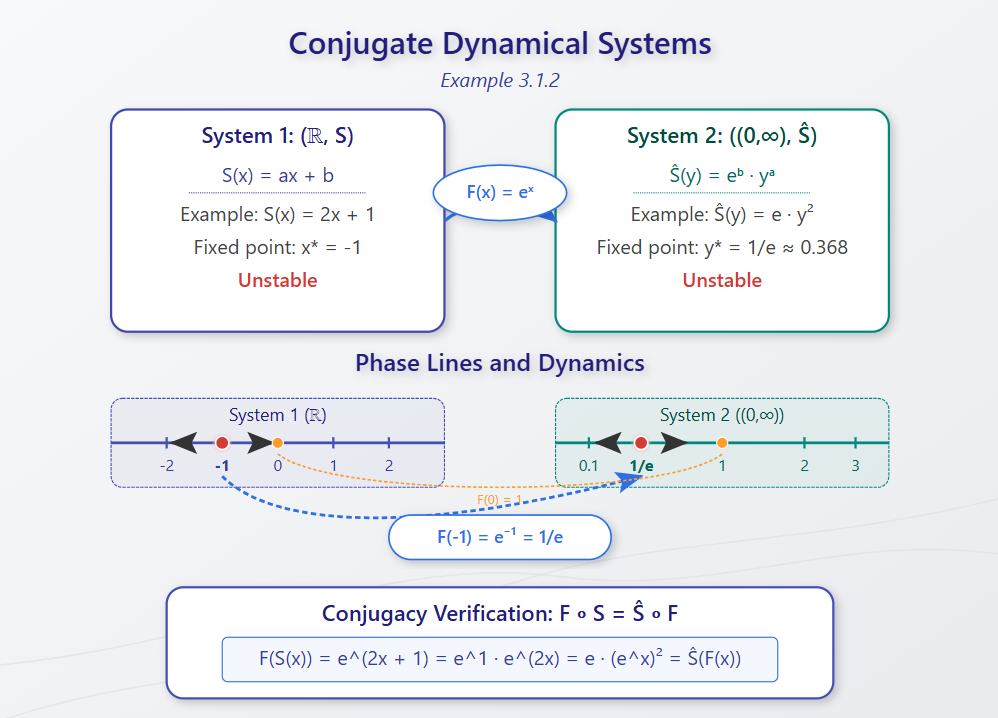
\includegraphics[width=0.68\linewidth]{image/Example 3.1.2.png}
       \caption{Caption}
       \label{fig:enter-label}
   \end{figure} 
\end{frame}

\begin{frame}{Order conjugacy}
\begin{definition}
    Consider two dynamical systems $(V,S)$ and $(\hat V, \hat S)$, where $V,\hat V$ are posets. We call these systems \textbf{order conjugate under $F$} if they are conjugate under $F$, and, $F$ is an order isomorphism.
\end{definition}
\end{frame}

\begin{frame}{Exercise 3.1.9.}
Prove that order conjugacy is an equivalence relation on the set of dynamical systems over partially ordered set.
\begin{proof}
    We denote $(V,S)\sim (\hat{V},\hat S)$ is they are order conjugate. We need to show this relation is reflexive, symmetric and transitive. 
    \begin{itemize}
        \item (Reflexivity) Let $F=Id$ which is a bijection. We have 
        $$
        F\circ S = S = S\circ F 
        $$
        Moreover, we have $F = F^{-1}$ is order preserving. Hence, 
        $$
        (V,S) \sim (V,S)
        $$
    \end{itemize}
\end{proof}
\end{frame}

\begin{frame}{Exercise 3.1.9 Continue}
\begin{proof}
        \begin{itemize}
        \item (Symmetry) Let $(V,S)\sim (\hat V,\hat S)$ under $F$. 
        \begin{itemize}
            \item $F$ is bijection implies $F^{-1}$ is bijection
            \item $F\circ S = \hat S\circ F\implies F^{-1} \circ \hat S = S\circ F^{-1}$ 
        \end{itemize}
        Hence, $(V,S)$ and $(\hat V,\hat S)$ are conjugate under $F^{-1}$.
        \begin{itemize}
            \item $F$ is order preserving with order preserving inverse implies $F^{-1}$ is order preserving with order preserving inverse
        \end{itemize}
        Hence, $F^{-1}$ is order isomorphism. Hence $(\hat V,\hat S)\sim (V,S)$
    \end{itemize}
\end{proof}
\end{frame}

\begin{frame}{Exercise 3.1.9 Continue}
\begin{proof}
    \begin{itemize}
        \item (Transitive) Let $(V_1, S_1)\sim (V_2,S_2)$ under $F$ and $(V_2,S_2)\sim (V_3, S_3)$ under $G$. 
        \begin{itemize}
            \item $F,G$ are bijective implies $H := (G\circ F)$ is bijective
            \item $F\circ S_1 = S_2\circ F, G\circ S_2 = S_3\circ G\implies  (G\circ F)\circ S_1 = G\circ S_2 \circ F = S_3\circ(G\circ F)$
        \end{itemize}
        Hence, $(V_1,S_1)$ and $(V_3,S_3)$ are conjugate under $H$.
        \begin{itemize}
            \item $F,G$ are order preserving with order perserving inverses
            \item $G\circ F$ are order preserving with order preserving inverses
        \end{itemize}
        Hence, $(V_1,S_1)\sim (V_3, S_3)$ under $(G\circ F)$.
    \end{itemize}
\end{proof}
    
\end{frame}

\begin{frame}{Lemma 3.1.3.}
If $(V,S)$ and $(\hat V,\hat S)$ are order conjugate under $F$, then $S$ is order stable on $V$ if and only if $\hat S$ is order stable on $\hat V$.
\begin{proof}
    $(\implies)$ Suppose $S$ is order stable on $V$. This implies
    \begin{itemize}
        \item[(S1)] $S$ has a unique fixed point $v^*\in V$
        \item[(S2)] $v\in V, v\precsim v^*\implies v\precsim Sv$ and $v\in V, v^*\precsim v\implies Sv\precsim v$
    \end{itemize}
    $(S1)$ implies $\hat S$ has a unique fixed point $\hat v^* : =F(v)\in \hat V$ by Proposition 3.1.2. Moreover we have
    \begin{itemize}
        \item For $\hat v:= F(v)\in \hat V, \hat v\le \hat v^*\underbrace{\implies}_{o.i.} v\precsim v^*\underbrace{\implies}_{S2} v\precsim Sv\underbrace{\implies}_{o.i.}Fv\le \underbrace{FSv = \hat S\hat v}_{conjugate}$
        
    \end{itemize}
    
    
\end{proof}
    
\end{frame}

\section{3.1.1.3 Isomorphic ADP}
\begin{frame}{Isomorphic ADP}
    In this section, we will see how one ADP can be transformed into another ADP (or ADPs are equivalent up to a transformation). \\
    \\
    Such transformation will result
    \begin{itemize}
        \item Simpler form of Bellman equation
        \item Tailored to solve for some problems (Exponential BE)
        \item etc. 
    \end{itemize}
\end{frame}
\begin{frame}{Definitions}
    \begin{definition}
        Let $(V,\mathbb{T})$ and $(\hat V,\hat{\mathbb{T}})$ be ADPs with policy sets $\mathbb{T}:= \{T_\sigma:\sigma\in\Sigma\}$ and $\hat{\mathbb{T}}:= \{\hat T_\sigma :\sigma \in\Sigma\}$. We call these ADPs \textbf{isomorphic} under $F$ if
        \begin{enumerate}
            \item $F$ is an order isomorphism from $V$ to $\hat V$
            \item these two ADPs have the same policy set $\Sigma$
            \item $(V,T_\sigma)$ and $(V,\hat T_\sigma)$ are order conjugate under $F$ for all $\sigma\in\Sigma$.
        \end{enumerate}
    \end{definition}
\end{frame}

\begin{frame}{Example 3.1.3. Fei et al. (2021) Exponential Bellman Equation}
    Exponential risk-sensitive Q-factor Bellman equation (ADP: $((0,\infty)^G,\mathbb{M})$)
    $$
    M_\sigma h = \exp (\theta r + \beta\ln P_\sigma h), \quad P_\sigma h(x,a):= \sum_{x'} h(x',\sigma(x')) P(x,a,x')
    $$
    Risk-sensitive Q-factor policy operator (ADP: $(\mathbb{R}^G, \mathbb{T})$)
    $$
    T_\sigma f = r+\frac{\beta}{\theta} \ln \bigg[P_\sigma \exp(\theta f)\bigg],\quad P_\sigma\exp(\theta f)(x,a):= \sum_{x'} \exp(\theta f(x',\sigma(x')) P(x,a,x')
    $$
\end{frame}

\begin{frame}{Example 3.1.3. Continue}
Let $\theta>0$, and 
$$
Fh = \exp(\theta h)
$$
is an order isomorphism from $\mathbb{R}^G$ to $(0,\infty)^G$.\\
\\
For conjugacy, we have
\begin{align*}
  (F\circ T_\sigma)(h) &= \exp\left(\theta (r+\frac{\beta}{\theta})\ln \bigg[P_\sigma \textcolor{red}{\exp(\theta h)}\bigg] \right)\\
  &= \exp\left(\theta r+\beta \ln P_\sigma (Fh) \right)\\
  &= (M_\sigma \circ F) (h)
\end{align*}
Hence, $((0,\infty)^G,\mathbb{M})$ and $(\mathbb{R}^G, \mathbb{T})$ are isomorphic
\end{frame}

\begin{frame}{Example 3.1.4. RDP}
Let $(\Gamma, V, B)$ and $(\Gamma, \hat V, \hat B)$ be two RDPs with identical state sapce $X$, action space $A$, and feasible correspondence $\Gamma$. Let $V = M^X,\hat V = \hat M^X$, where $M,\hat M\subset \mathbb{R}$. If there exists an order isomorphism $\varphi$ from $M$ to $\hat M$ such that
$$
B(x,a,v) = \varphi^{-1} [\hat B(x,a,\varphi\circ v)] \quad\text{for all $v\in V$ and $(x,a)\in G$}
$$
then $(V,\mathbb{T})$ and $(\hat V,\hat{\mathbb{T}})$ are isomorphic. From exercise 3.1.2, $F$ is an order isomorphism from $V$ to $\hat V$, and
$$
T_\sigma  = F^{-1} \circ \hat T_\sigma \circ F
$$
\end{frame}


\begin{frame}{Lemma 3.1.4.}
\begin{lemma}
    Isomorphism between ADPs is an equivalence relation on the set of ADPs.
\end{lemma}
\begin{proof}
    Let $\mathbb{A}$ be the set of ADPs. We denote $(V_1,\mathbb{T}_1)\cong(V_2, \mathbb{T}_2)$ if there are isomorphic. We need to prove that $\sim$ is reflexive, symmetric and transitive.
    \begin{itemize}
        \item (Reflexivity) Let $(V,\mathbb{T})\in \mathbb{A}$, as the ADP has the same policy set as itself and by Exercise 3.1.9, we get reflexivity.
        \item (Symmetry) Let $(V_1,\mathbb{T}_1)\cong(V_2, \mathbb{T}_2)$, then they have the same policy set. We use Exercise 3.1.9 get symmetry
        \item (Transitivity) Let $(V_1,\mathbb{T}_1)\cong(V_2, \mathbb{T}_2)$ and $(V_2,\mathbb{T}_2)\cong(V_3, \mathbb{T}_3)$, hence these three ADPs have the same policy set. We use Exercise 3.1.9. get transitivity.
    \end{itemize}
\end{proof}
\end{frame}

\section{3.1.1.4 Isomorphisms and Optimality}
\begin{frame}{Isomorphisms and Optimality}
    
\end{frame}

\begin{frame}{Notations}
    We take
    \begin{itemize}
        \item $(V,\mathbb{T})$ and $(\hat V,\hat{\mathbb{T}})$ be two ADPs
        \item $\mathbb{T} := \{T_\sigma: \sigma\in\Sigma\}$; $\hat{\mathbb{T}}:=\{\hat T_\sigma: \sigma \in\Sigma\}$
        \item $v_\sigma (resp. \hat v_\sigma)$ be the unique fixed point of $T_\sigma (resp. \hat T_\sigma)$
        \item $T(resp. \hat T)$ be the Bellman operator of $(V,\mathbb{T})$ (resp. $(\hat V,\hat{\mathbb{T}})$)
        \item $v^*$ (resp. $\hat v^*$) be the value function of $(V,\mathbb{T})$ (resp. $(\hat V,\hat{\mathbb{T}})$)
    \end{itemize}
\end{frame}

\begin{frame}{Theorem 3.1.5.}
\begin{theorem}
    If $(V,\mathbb{T})$ and $(\hat V,\hat{\mathbb{T}})$ are isomorphic under $F$, then
    \begin{enumerate}
        \item $\sigma$ is $v$-greedy  for $(V,\mathbb{T})$ $\iff$ $\sigma$ is $Fv$-greedy for $(\hat V,\hat{\mathbb{T}})$
         \item $\sigma$ is optimal  for $(V,\mathbb{T})$ $\iff$ $\sigma$ is optimal for $(\hat V,\hat{\mathbb{T}})$
        \item Regularity, well-posedness, and order stability is preserved under isomorphism.
    \end{enumerate}
\end{theorem}
    
\end{frame}
\end{document}
